\chapter{シーケンシャルデータの処理}

ドメイン・エンティティやエンティティまたは値のコレクションができたら、アプリケーションの要件を満たすために、質問に答えたり、データを新しい形に変換したりできるようにする必要があります。しかし、Clojureはデータの集合体レベルで考えることを推奨しており、コレクション全体に一度に変換を適用します。

Clojureは、単一のデータ構造を操作する広範な関数群を構築するのではなく、その変換のすべてをシーケンス抽象化に基づいて構築します。シーケンスは、Clojureの最も重要な2つの部分、すなわち、不変のコレクションと変換ライブラリをつなぐ重要な抽象化である。

抽象化とは、値のシーケンシャルなソースをトラバースするための最も重要な側面(最初の値を取得し、残りをシーケンスとして取得し、終了をチェックする手段)だけが含まれていることを意味します。シーケンスが実現されると、その値はキャッシュされ、実現状態に関わらずシーケンスは不変である。この単純な抽象化により、変換ライブラリのほぼすべての関数と、すでに見たことのあるすべてのコレクションを接続するのに十分である。

さらに重要なことは、シーケンス抽象化の参加者とその上で動作する関数の両方がオープンシステムであり、この組み合わせが2次元(より多くのデータとより多くの関数)的に拡張可能であることです。どの関数でもどのデータでも接続できることは、Clojureプログラム内、そしてClojureプログラム間で非常に大きな再利用性を可能にし、Clojureプログラムを簡潔かつ表現力豊かにする重要な要因です。

シーケンスは当初からClojureの一部でした。Clojure 1.7はトランスデューサーの概念を導入しています。これはシーケンシャル処理をさらに進化させたもので、入力の反復、変換の適用、出力の生成の概念を分割しています。これらの断片を分離することで、トランスデューサーはさらに幅広いコンテキストで逐次変換の再利用を可能にします。この章を通して、シーケンスとトランスデューサーの比較と、それぞれを最大限に活用する方法を紹介します。

おそらく、シーケンス変換の最も一般的な種類の1つは、シーケンス内のすべての値に関数を適用して新しいシーケンスを生成するという考え方で、私たちはそこから始めましょう。続いて、その他の一般的な変換として、値への還元、フィルタリング、シーケンスの一部の削除、グループ化、ソート、重複の削除について見ていきます。最後に、これらの変換をすべて組み合わせて、変換パイプラインを作成する方法について説明します。 

\section{値のマッピング}

アプリケーションの中でデータが移動するとき、ある部分が別の形でデータを必要とすることはよくあることです。あるサブシステムは、30列のスプレッドシートから30個のキーを持つ汎用マップにデータをインポートする。別のサブシステムでは、5列のデータをエンティティの形で必要とし、さらに別のシステムでは、一連のエンティティから1つのフィールドのみを必要とし、計算を実行したり画面に表示したりします。

これらのユースケースはすべて、シーケンシャルなソースにある値をある形式から別の形式に変換する必要があります。Clojureでは、map関数はシーケンスの各要素に関数を適用して、その結果の新しいシーケンスを生成するために使用されます。

例えば、宇宙シミュレーションの各惑星エンティティの軌道周期を抽出して画面に表示する必要があるとします。入力は惑星のベクターであり、これはシーケンス、つまり論理的には値のリストとして扱われます。

このシーケンシャルな惑星の集合を、各惑星の軌道周期のシーケンシャルな集合に変換する必要がある。軌道周期とは、惑星が太陽の周りを完全に1周するのにかかる時間である。例えば、地球の場合、公転周期は約365.25日である。

$$
\mu = GM
$$

$$
T = 2 \pi \sqrt{\frac{a^3}{\mu}}
$$

任意の惑星の公転周期を計算する関数を書くことができる。この関数の詳細を理解することは、特に重要ではありません。(もし興味があれば、ここにその方程式を示す。Tは惑星の公転周期、$μ$は標準的な重力パラメータです)。

この値は、惑星だけでなく、中心星の質量にも依存する。公転周期を計算する関数は、惑星と恒星の質量を引数として受け取り、公転周期を返す。



\begin{lstlisting}[numbers=none]
(defn semi-major-axis
  "The planet's average distance from the star"
  [p]
  (/ (+ (:aphelion p) (:perihelion p)) 2))

(defn mu [mass] (* G mass))

(defn orbital-period
  "The time it takes for a planet to make a complete
  orbit around a mass, in seconds"
  [p mass]
  (* Math/PI 2
    (Math/sqrt (/ (Math/pow (semi-major-axis p) 3) (mu mass)))))
\end{lstlisting}

さて、変換関数ができたので、それを使って惑星のコレクションを公転周期のコレクションに変換しなければなりません。Clojureのマップ関数は、惑星のベクターに変換関数を適用して、連続したソース内のすべての値を新しい値に「マップ」する方法です。

1つの引数(値)を取り、新しい値を返す変換関数が必要です。しかし、\texttt{orbital-period}関数は2つの引数を取る関数なので、今ある関数を正しい形(1つの引数)の変換関数にラップする必要があります。これは、定数値(太陽質量)が現在の関数スコープで利用可能な無名関数を使用することでしばしば行われる。

\begin{lstlisting}[numbers=none]
(defn orbital-periods
  "Given a collection of planets, and a star, return the
  orbital periods of every planet."
  [planets star]
  (let [solar-mass (:mass star)]
    (map (fn [planet] (orbital-period planet solar-mass))
         planets)))
\end{lstlisting}

この例では、惑星のコレクションと星を受け取り、星から太陽質量を取り出しています。そして、惑星を受け取り、その惑星と太陽質量を用いてorbital-period関数を呼び出す無名関数でmapを呼び出すことができます。map関数は、この関数をすべての惑星に適用しながらコレクションを走査し、結果を一連のシーケンスにまとめて最後に返します。

mapが何をしているのか、コレクションの世界からシーケンスの世界へどのように入り込んでいるのか、もっと詳しく見ていきましょう。


\subsection{シーケンス処理}

 mapの仕事は、シーケンスのすべての値に関数を適用することである。ここでは Clojureがこの関数を実装する方法の簡略版です。このバージョンを \texttt{simple-map} と呼ぶことにします。


\begin{lstlisting}[numbers=none]
(defn simple-map
  "Map f over the elements of coll."
  [f coll]
  (when (seq coll)
    (cons (f (first coll))
          (simple-map f (rest coll)))))
\end{lstlisting}

この実装はClojureのシーケンスAPIを使って書かれており、主に\texttt{seq}, \texttt{first}, \texttt{rest}, \texttt{cons}関数から構成されています。\texttt{seq}関数は、コレクションが少なくとも1つの要素からなるシーケンスであるかどうかを尋ねます。もしそうなら,それが返され,そうでなければ,nilが返される.この結果は真か偽かを表すので、この関数はしばしば終了の条件チェックに使われる。

マッピングされるコレクションがより多くの要素を持つ場合、\texttt{cons}関数を適用する。\texttt{cons}関数は、値を含むセルと、次のセルへのポインタを構成する。これは典型的なリンクリストのデータ構造であり、値を含む一連のセルである。最初のセルの値は、変換関数fをコレクション内の最初の値に適用したものとして定義される。残りのセルは、同じ関数と入力コレクションの残りを渡して、この関数を再帰的に呼び出すことによって定義される。

この再帰的なシーケンスの定義は、シーケンシャルなコレクション(リストまたはベクタ)に適用されるが、そのデータ構造の実装方法の詳細には一切依存しない。シーケンスAPIを実装するためには、参加者(participant)は次の要素が存在するかどうかをチェックし、最初の要素を返し、残りの要素に対して新しい実体を返すことができればよいのである。つまり、シーケンスとはコレクションの論理的な見方である。

軌道周期の例では、シーケンシャルなコレクションやシーケンスAPIの他の実装を渡しても、\texttt{map}は動作する。シーケンスの抽象化により、汎用的な\texttt{map}関数が様々なデータソースで動作するようになった。

一般にシーケンス関数は、seqable(\texttt{seq}を適用するとシーケンスを生成できるもの)を入力として受け取り、同じものを返すと考えられています。しかし、この場合の結果は永続的なリストとなり、関数に渡されたベクトルほど高速でもメモリ効率も良くはありません。Clojureはこの特殊なケースのために、特別なmapv関数を提供します。mapv関数はmapと使い方は同じですが、特にベクトルを受け取って返します。

これは、ほとんどのシーケンス関数の典型的な側面を強調しています。入力ソース(シーケンス対ベクトル)の反復、変換の適用(\texttt{f}関数の適用)、結果に対する何らかの処理(リストの構築またはベクトルの構築)を組み合わせています。

この3つを組み合わせると、シーケンスの使い方が制限されます。しかし シーケンス入力は抽象化されたものであり,事実上あらゆるソースで実装可能である.同様に,この関数は出力シーケンスしか生成しないので,コレクションに挿入したり,通信チャネルに値を渡したりするには,別のバージョンが必要になる.これらの部品を分解するために、トランスデューサーが導入された。

\subsection{トランスデューサー}

トランスデューサの定義では、入力値がどこから来て、その出力がどのように使われるかを指定することを避け、代わりにトランスデューサが行う実際の作業のみを定義します。\texttt{map}の場合、トランスデューサの仕事は関数がすべての要素に適用されるようにすることです。その本質は、入力要素がコレクション、シーケンス、ソケット、キューのどれであっても、また、出力がコレクションに追加されるかファイルに保存されるかにかかわらず、同じです。

トランスジューサの実装はやや複雑なので説明しませんが、どのように作成され適用されるかを見ることは重要です。マップトランスジューサを作るには、\texttt{map}を呼び出すときに入力コレクションを省略します。

\begin{lstlisting}[numbers=none]
(defn orbital-period-transformation
  "Create a map transformation for planet->orbital-period."
  [star]
  (map #(orbital-period % (:mass star))))
\end{lstlisting}

この変換は、様々な入力ソースと出力条件に対して使用することができる。前の版の\texttt{map}と同様の出力シーケンスを生成するために、この変換とシーケンス関数を使用することができます。

\begin{lstlisting}[numbers=none]
(defn orbital-periods
  [planets star]
  (sequence (orbital-period-transformation star) planets))
\end{lstlisting}

\texttt{mapv}版のような出力ベクトルを作成する場合は、以下のようにします。

\begin{lstlisting}[numbers=none]
(defn orbital-periods
  [planets star]
  (into [] (orbital-period-transformation star) planets))
\end{lstlisting}

あるいはリストを作成する。

\begin{lstlisting}[numbers=none]
(defn orbital-periods
  [planets star]
  (into () (orbital-period-transformation star) planets))
\end{lstlisting}

\texttt{sequence}と\texttt{into}を用いた\texttt{orbital-periods}は、要素の実現方法が異なるため、遅延の概念に関わる。




\subsection{遅延性}

ほとんどのClojureシーケンス関数は、関数が評価されるときに変換を実行しない、遅延シーケンスを生成します。その代わり、遅延シーケンスは、シーケンスの消費者が必要とするときだけ評価されます。オリジナルのシーケンス版である \texttt{map} とシーケンス付きトランスデューサーは、どちらも必要に応じて計算される遅延シーケンスを生成します。

遅延シーケンスは、決して計算される必要のない作業を避けることができるという点で有用です。この場合、軌道周期の遅延シーケンスを消費するコードがなければ、計算する必要はないでしょう。遅延シーケンスは、フィボナッチ・シーケンスや素数シーケンスのような無限の値の並びを表現するのにも便利です。我々は、計算のためにそれらすべてを見ることは決してない(ありえない)。しかし、無限シーケンスとして定義することで、目的に応じて必要な数だけ取ることができる。

これに対して、\texttt{into} は出力全体を熱心に計算し、それを返す関数である。熱心な計算が便利なのは、計算がいつ行われるかを簡単に推論できるようになるからです。これにより、トランスデューサーで使用されるリソースの管理や廃棄が容易になったり、計算が行われるタイミングを正確に管理することができます。

さらに、\texttt{into}で行われる熱心な計算は、しばしばメモリと時間の両面でより効率的です。シーケンスは計算された値をキャッシュしますが、トランスデューサーの熱心なアプリケーションは、中間値を割り当てることなくソースコレクションに対して実行できることがよくあります。

\texttt{into}関数は、より一般的な\texttt{reduce}関数で実装されており、入力コレクションを値に還元します。









\begin{lstlisting}[numbers=none]

\end{lstlisting}




 % Mapping Values
\section{値への還元}

\texttt{reduce}関数は、蓄積された値とコレクションの次の要素に関数を繰り返し適用することで、コレクションを値に還元する関数です(オプションの初期値を使用)。\texttt{into}関数は、コレクションを単純な値ではなく、別のコレクションに還元する特殊なケースです。

例えば、宇宙シミュレーションで、太陽系のすべての惑星にある月の総数を計算することを考えてみましょう。まず、各惑星の月の数を抽出し(マッピング変換)、それらを\texttt{+}関数で一つの値(合計)に還元する必要があります。\texttt{reduce}関数は、収集変換と削減のステップを組み合わせるためによく使われる。

\texttt{map}と\texttt{reduce}を使って、惑星の集合の総和を計算することができる。



\begin{lstlisting}[numbers=none]
(defn total-moons
  [planets]
  (reduce + 0 (map :moons planets)))
\end{lstlisting}

この関数は、各 \texttt{Planet} レコードに適用する関数として \texttt{:moons} というキーワードを使用して、惑星をマッピングします。その結果、各惑星の月の数を表す数値の列が生成されます。

次に、\texttt{reduce}はそれらの要素にそれぞれ+関数を適用し、初期蓄積値として0から始めます。

\texttt{reduce}はシーケンスではなく、値を生成するため、イーガーとなります。そのため、計算は\texttt{reduce}が実行されたときに行われます。

この変換は,トランスデューサーと類似の関数である\texttt{transduce}を使って計算することもできます.この関数は\texttt{reduce}とは異なり,入力ソースの各要素に適用するトランスデューサと,変換の出力値をどうするかを決定する\texttt{reduce}関数の2つの関数を受け取ります.トランスデューサーは意図的に、入力がどのように供給されるか(ここではソースコレクションから)と、その後に入力に対して何が行われるかの両方から変換を切り離すことを思い出してください。



\begin{lstlisting}[numbers=none]
(defn total-moons
  [planets]
  (transduce (map :moons) + 0 planets))
\end{lstlisting}


 % Reducing to a Value
\section{値のフィルタリングと削除}

惑星のコレクションではなく、太陽系内の全エンティティのコレクションを渡されることもある。その場合、月の総数を計算するには、惑星だけをフィルタリングして月の数を抽出し、月の総数を計算する必要がある。まずは配列を使ってどのように見えるか見てみましょう。


\begin{lstlisting}[numbers=none]
(defn planet?
  [entity]
  (instance? Planet entity))

(defn total-moons
  [entities]
  (reduce + 0
    (map :moons
      (filter planet?
        entities))))
\end{lstlisting}





 % Filtering and Removing Values
\section{takeとdrop}

述語に基づいてコレクションのサブセットを構築する代わりに、コレクションの先頭を取得または削除することがしばしば有用である。Clojureでは、\texttt{take}と\texttt{drop}関数がこれを達成することができます。例えば、外部ソースから太陽系エンティティのシーケンスを受け取る場合、次のような関数で結果のn番目のページを取得することができます。


\begin{lstlisting}[numbers=none]
(defn nth-page
  "sourceのn番目(0ベース)のpageに対して、page-sizeまでの結果を返す"
  [source page-size page]
  (->> source
       (drop (* page page-size))
       (take page-size)))
\end{lstlisting}

この関数は、まず要求されたページまでのページ数を落とし、次に要求されたページの集合を取り込む。この関数はシーケンスを使用し,要求されたページの結果を超える要素は実現しない.トランスデューサのフォームは、早期終了を知らせるために\texttt{reduced}を使用し、また要求された範囲を超えた結果を実現しないようにします。

ページを返すだけでなく、そのページと残りのコレクションの両方をさらなる処理のために必要とする場合もあります。split-at ヘルパー関数は \texttt{take} と \texttt{drop} の両方を実行し、両方をタプルとして返します。


\begin{lstlisting}[numbers=none]
(defn page-and-rest
  [source page-size]
  (split-at page-size source))
\end{lstlisting}

これは、最初のページと、最初のページ以外のすべてのベクターを返します。さらに処理を進めると、最初のページ以降の結果に対して再びこれを呼び出すことができる。

また、\texttt{take}と\texttt{drop}はカウントではなく述語で動作するバージョン、\texttt{take-while}と\texttt{drop-while}も使用できる。\texttt{split-with}関数は\texttt{split-at}と等価な述語です。

\texttt{take}と\texttt{drop}関数で要素のサブセットを選択する前に、コレクション内の要素の順序を指示するためにソートを組み合わせることはしばしば有用である。




 % Take and Drop
\section{ソートと重複排除}

最も基本的なソート機能は \texttt{sort} で、デフォルトのコンパレータまたは必要に応じてカスタムのコンパレータでソートすることができます。例えば、これはアルファベット順で最初の5つの惑星名を取得します。


\begin{lstlisting}[numbers=none]
(take 5 (sort (map (:name planets))))
\end{lstlisting}

この例では、惑星の名前を取得し、その名前をソートしています。しかし、しばしば、元の実体を惑星名で並べ替えたいことがある。つまり、値を取り出すのではなく、各要素に適用される関数でソートしたいのです。これは\texttt{sort-by}で実現できる。


\begin{lstlisting}[numbers=none]
(take 5 (sort-by :name planets))
\end{lstlisting}

 % Sorting and Duplicate Removal
\section{値のグループ化}

便利な\texttt{group-by}関数は、述語に基づいてデータをグループ化し、述語の結果とその結果にマッチするすべてのシーケンスのマップを返すことができます。例えば、惑星の最初の文字でインデックスを作成することができます。



\begin{lstlisting}[numbers=none]
(defn index-planets
  [planets]
  (group-by #(first (:name %)) planets))
\end{lstlisting}

この関数は、\texttt{E}, \texttt{J}, \texttt{M}, \texttt{N}, \texttt{S}, \texttt{U}, \texttt{V}をキーとするマップを返す。各値は、地球、木星、火星と水星、海王星、土星、天王星、金星の惑星エンティティのシーケンスである。

\texttt{group-by}の一般的な使用方法の1つは、含むコードで両方が必要な場合に\texttt{true}と\texttt{false}のキーのマップを返す述語と組み合わせて使用することです。

例えば、月のある惑星と月のない惑星を分けたい場合、述語は次のようになります。


\begin{lstlisting}[numbers=none]
(defn has-moons?
  [planet]
  (pos? (:moons planet)))
\end{lstlisting}

この述語は、マップ上で惑星を2つのバケツに分けるために使われる。


\begin{lstlisting}[numbers=none]
(defn split-moons
  [planets]
  (group-by has-moons? planets))
\end{lstlisting}

Clojureでシーケンシャルなデータを処理する一般的な方法のほとんどを示したので、より大きな例のコンテキストでそれがどのように見えるかを見てみましょう。 % Grouping Values
\section{すべてをまとめる}

多くの場合、シーケンシャルデータの処理は同じようなパターンで行われます。

\begin{enumerate}
\item  どんな質問をしようとしているのかを把握する。このステップは、問題領域やビジネス領域に位置するため、最も困難な場合が多い。明確な質問があれば、Clojureはあなたが持っているデータを処理して答えを出すためのツールを提供します。それが次の3つのステップです。
\item  データをフィルタリングして、不要な要素を取り除く。
\item 要素を目的の形に変換する。
\item 変換された要素を答えに還元する。
\end{enumerate}


ショッピングカートの例で説明しましょう。オンラインストアでは、カタログ、つまり販売する商品のリストがあります。これらの商品は部門ごとに分けられています。顧客はそれらをカートに入れ、チェックアウトする。このプロセスで、請求記録が作成されます。あなたの顧客は、部門別の売上を要約したレポートを要求しています:すべての決済されたカートについて、部門ごとの総売上はいくらですか?

ドメインモデルは次のとおりです。


\begin{lstlisting}[numbers=none]
(require '[money :refer [make-money +$ *$]])

(defrecord CatalogItem [number dept desc price])
(defrecord Cart        [number customer line-items settled?])
(defrecord LineItem    [quantity catalog-item price])
(defrecord Customer    [cname email membership-number])
\end{lstlisting}

何度もチェックアウトを繰り返すと、カートには\texttt{\#Cart}レコードのベクターが含まれることがあります。


\begin{lstlisting}[numbers=none]
[#Cart{:number 116,
       :customer #Customer{:cname "Danny Tanner",
                           :email "danny@fullhouse.example.com",
                           :membership-number 28374},
       :line-items [
         #LineItem{:quantity 3,
                   :catalog-item #CatalogItem{:number 664,
                                              :dept :clothing,
                                              :desc "polo shirt L",
                                              :amount 2515 :currency :usd},
                   :price #Money{:amount 7545
                                 :currency :usd}
         #LineItem{:quantity 1,
                   :catalog-item #CatalogItem{:number 621,
                                              :dept :clothing,
                                              :desc "khaki pants",
                                              :price #Money{:amount 3500
                                                            :currency
                                                            :usd},
                   :price #Money{:amount 3500
                                 :currency :usd}
                    ],
       :settled? true}, ,,, ]
\end{lstlisting}


これはかなり大きなデータ構造で、次の図のようなクラス図で理解するのが分かりやすいかもしれません。

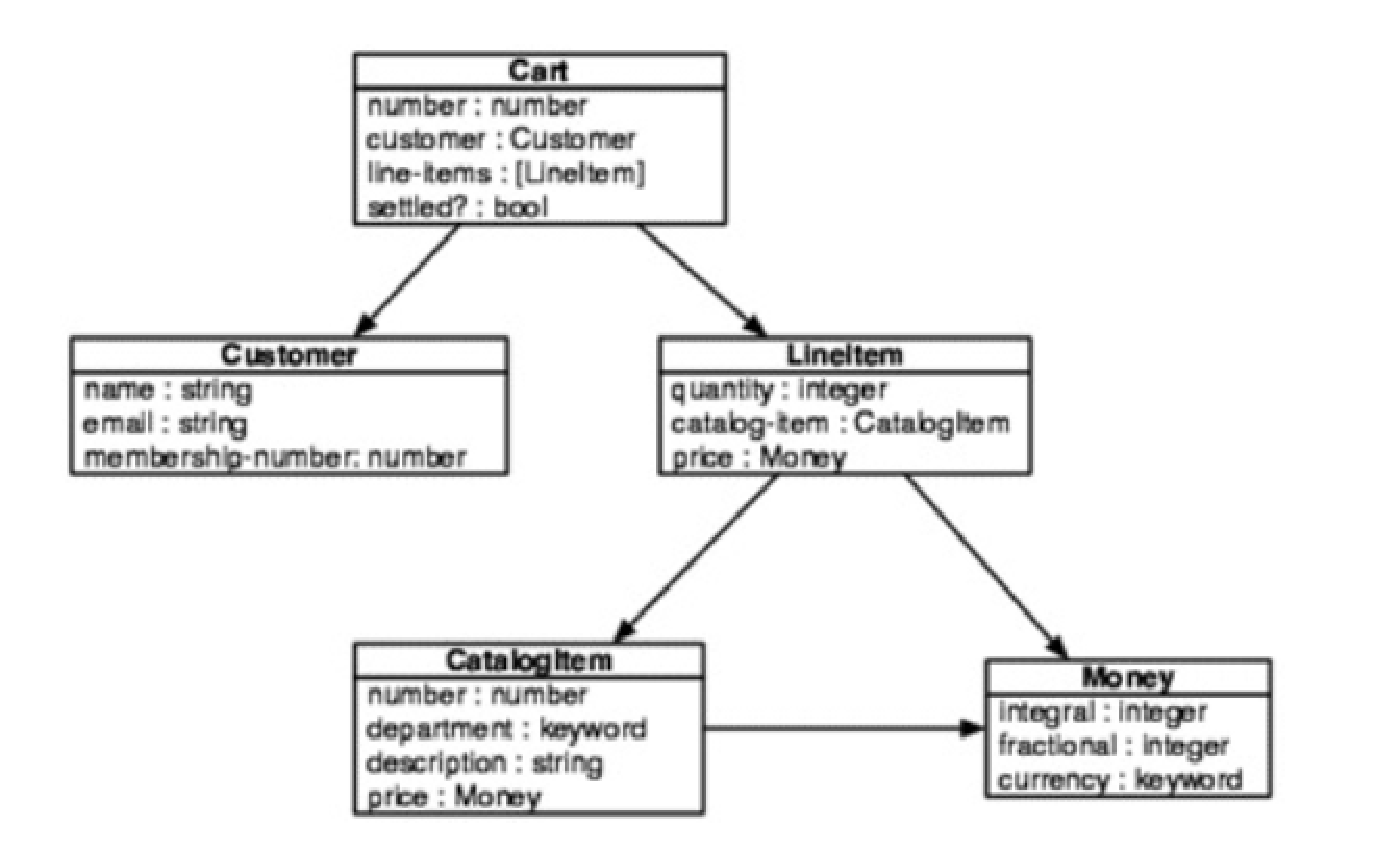
\includegraphics[width=12cm]{fig_03_001.eps}

私たちが求めているのは、もっとシンプルな、部門と金額の対応表です。



\begin{lstlisting}[numbers=none]
{:clothing #Money{:amount 2386424, :currency :usd}
 :toys     #Money{:amount 1163277, :currency :usd}
 ,,, }
\end{lstlisting}

カートの中身から目的の出力まで、順を追って説明しましょう。まず最初にやるべきことは、気になるデータを見つけることです。

\subsection{選択}

シーケンス処理の選択ステップでは、興味のある要素だけを含む部分シーケンスを識別して作成します。カートデータに対してフィルタを使用することで、その要素を取得することができます。

レポートを作成する際、決済されたカートのみを考慮します。決済されるまでは、実際の収益ではなく、潜在的な収益に過ぎないからです。まず、filterを使用してリストのサイズを小さくします。



\begin{lstlisting}[numbers=none]
(defn revenue-by-department [carts]
  (->> (filter :settled? carts)
       ,,,))
\end{lstlisting}

キーワード \texttt{:settled?} を関数として使用すると、 \texttt{:settled?} が\texttt{true}でないカートをすべてフィルタリングすることができます。

\subsection{トランスフォーメーション}

これで一連の決済カートが揃ったので、部門別に収益を分離することができるようになりました。カートは一切必要なく、品目とカタログ品だけが必要なことがわかります。今は一歩ずつ進めていきましょう。次のステップは、すべてのラインアイテムのシーケンスを作成することです。


\begin{lstlisting}[numbers=none]
(defn revenue-by-department [carts]
  (->> (filter :settled? carts)
       (mapcat :line-items)
       ,,,))
\end{lstlisting}

\texttt{(mapcat :line-items ,,)} の結果は、このようになります。


\begin{lstlisting}[numbers=none]
[#LineItem{:quantity 3,
           :catalog-item #CatalogItem{:number   664,
                                      :dept  :clothing,
                                      :desc "polo shirt L",
                                      :price #Money{:amount 2515
                                                    :currency :usd}},
           :price #Money{:amount   7545
                         :currency :usd}},
 #LineItem{:quantity 1,
           :catalog-item #CatalogItem{:number 621,
                                      :dept :clothing,
                                      :desc "khaki pants",
                                      :price #Money{:amount 3500
                                                    :currency :usd}},
           :price #Money{:amount   3500
                         :currency :usd}}, ,,, ]
\end{lstlisting}

\texttt{mapcat}関数は、行項目ベクターの内容を集積したものを構築する。

\begin{itembox}[l]{mapcatとmap + flattenの使い分け}
\texttt{mapcat}の代わりに、\texttt{map}と\texttt{flatten}を併用することで、同様の結果を得ることができます。\texttt{flatten}を使いたくなったら、一歩戻って、そもそも\texttt{flatten}する必要がある構造を作らないようにしましょう。最も一般的なのは、\texttt{map}ではなく\texttt{mapcat}を使うことです(\texttt{map}と\texttt{concatenate}を行うため)。
\end{itembox}

次のステップは、各ラインアイテムから、カタログアイテムの \texttt{:dept} 値とラインアイテムの親の \texttt{:price} 値という気になるデータのマップを抽出することである。これは \texttt{map} と \texttt{line-summary} ヘルパー関数によって行われます。



\begin{lstlisting}[numbers=none]
(defn- line-summary
  "CatalogItem を持つ LineItem が与えられた場合、
   CatalogItem の :dept を :dept、LineItem の 
   :price を :total として含むマップを返します。"
  [line-item]
  {:dept (get-in line-item [:catalog-item :dept])
   :total (:price line-item)})

(defn revenue-by-department [carts]
  (->> (filter :settled? carts)
       (mapcat :line-items)
       (map line-summary)
       ,,,))
\end{lstlisting}

あと少しです。これで、報告する必要のあるデータのみを含む一連のマップができました。


\begin{lstlisting}[numbers=none]
[{:dept :clothing :total #Money{ ,,, }
 {:dept :clothing :total #Money{ ,,, }
 {:dept :toys     :total #Money{ ,,, }
 {:dept :kitchen  :total #Money{ ,,, }
 {:dept :toys     :total #Money{ ,,, }]
\end{lstlisting}

ここから、\texttt{group-by}を利用して、部門をキー、一連のサマリーを値とするマップを構築することができる。


\begin{lstlisting}[numbers=none]
(defn revenue-by-department [carts]
  (->> (filter :settled? carts)
       (mapcat :line-items)
       (map line-summary)
       (group-by :dept)
       ,,,))
\end{lstlisting}

この時点で、私たちのデータはこのようになっています。


\begin{lstlisting}[numbers=none]
{:clothing [{:dept :clothing :total #Money{},
            {:dept :clothing :total #Money{}, ,,,]
 :toys     [{:dept :toys     :total #Money{},
            {:dept :toys     :total #Money{}, ,,,]
 :kitchen  [{:dept :kitchen  :total #Money{}, ,,,]}
\end{lstlisting}

\texttt{:total}の\texttt{\#Money\{\}}の値のベクトルでサマリーを置き換えるという余分なステップを踏むこともできますが、それは不要です。その代わりに、最後のステップである、これらの値の要約に移りましょう。

\subsection{Reduction}

line-summary関数と同様に、各部門の集計を行う関数を定義して、削減処理で利用できるようにしたいと思います。


\begin{lstlisting}[numbers=none]
(require '[money :refer [make-money +$ *$])

(defn- dept-total
  [m k v]
  (assoc m k (reduce +$ (map :total v))))

(defn revenue-by-department [carts]
  (->> (filter :settled? carts)
       (mapcat :line-items)
       (map line-summary)
       (group-by :dept)
       (reduce-kv dept-total)))
\end{lstlisting}

断片的な\texttt{dept-total}関数の中に、通常のシーケンス処理パイプラインの縮図を見ることができます。この場合、\texttt{map}はシーケンスの各要素から\texttt{:total}を選択し、\texttt{reduce +\$}はそれを集計します。

\texttt{thread-last} マクロを使用した \texttt{dept-total} の代替実装は、読みやすいと思われます。


\begin{lstlisting}[numbers=none]
(defn- dept-total*
  [m k v]
  (assoc m k (->> (map :total v)
                  (reduce +$))))
\end{lstlisting}

以上です。最初のカートのベクトルを部門別の収益マップに落とし込みました。最終的なデータは、約束通り、このような形になりました。


\begin{lstlisting}[numbers=none]
{:clothing #Money{},
 :toys     #Money{},
 :kitchen  #Money{}, ,,, }
\end{lstlisting}

このセクションで行ったデータパイプラインは、\texttt{select}、\texttt{transform}、\texttt{reduce}という極めて典型的なものです。これはシーケンス処理の一単位と考えた方がよいかもしれません。\texttt{dept-total}関数で見たように、1つのシーケンス処理の単位が他の単位全体を包むことができるのです。練習を重ねるうちに、スムーズなパイプラインを作ることが反射的にできるようになるはずです。

もう一つ重要なことは、\texttt{revenue-by-department}関数で\texttt{thread-last}マクロ(\texttt{->>})を使っていることから明らかなように、シーケンスはプロセスの各段階に出入りしていることです。実際、最初の3つのステップ(\texttt{filter}, \texttt{mapcat}, \texttt{map})において、開始シーケンスの各要素は、次の要素が始まる前に3つのステップをすべて成功させることができ、結果は同じになるのです。これらのステップでは、前や後に続くものを考慮することなく、一度にシーケンスの単一の要素に対して操作を行います。これは、パイプラインのこの部分にトランスデューサを使用することも選択肢の一つであることを示す良い手がかりとなります。 % Putting It All Together
\section{まとめ}

ClojureコレクションはClojureデータの不変のベースを提供し、シーケンスはコレクションと他の順次トラバース可能なデータソースの両方の上に重要な抽象化を提供します。シーケンス関数とトランスデューサの両方を使ったシーケンシャルデータの最も一般的な処理方法を示しました。

トランスデューサーは、シーケンス処理モデルを、ソースの反復処理、変換、出力処理に分割し、それぞれを独立して変更できるようにすることで、より良いパフォーマンスとより多くの再利用性を獲得しています。入力ソースにトランスデューサを適用する3つの一般的な方法として、\texttt{sequence}、\texttt{into}、\texttt{transduce}の使い方を見ました。今後の章では、これらと同じトランスデューサー関数を \texttt{core.async} チャンネルに適用する方法も紹介します。

さて、ドメインをモデル化し、ドメインエンティティをコレクションにグループ化し、それらを処理したところで、スレッドと時間をまたぐ状態の連携を開始する方法を検討する必要があります。 % Wrapping Up
